\section{Pointer to Array}
\label{sec:structs}
\begin{frame}<beamer>
    \frametitle{Outline}
    \tableofcontents[currentsection]
\end{frame}

\begin{frame}{An Overview: Pointer to Array (1)}
\begin{figure}
	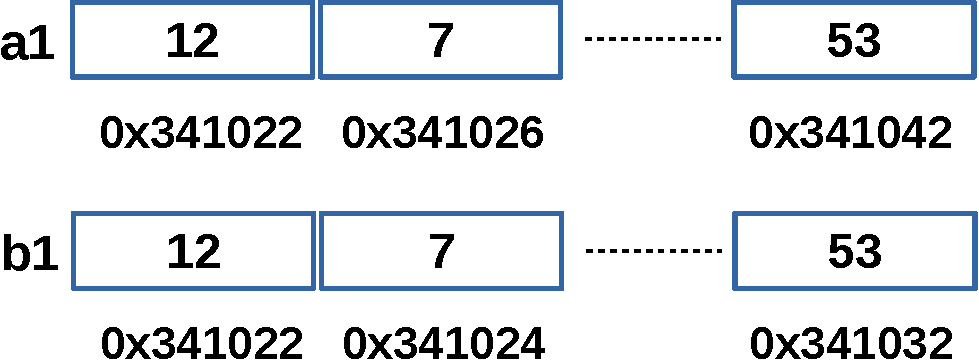
\includegraphics[width=0.68\linewidth]{figs/array1.pdf}
	\caption{Two typical arrays of \textcolor{blue}{int} type.}
\end{figure}
\begin{itemize}
	\item {Array is a continuous memory block}
	\item {It has a starting address}
	\item {It has a length}
	\item {It has a name}
\end{itemize}
\end{frame}

\begin{frame}[fragile]{An Overview: Pointer to Array (2)}
\begin{figure}
	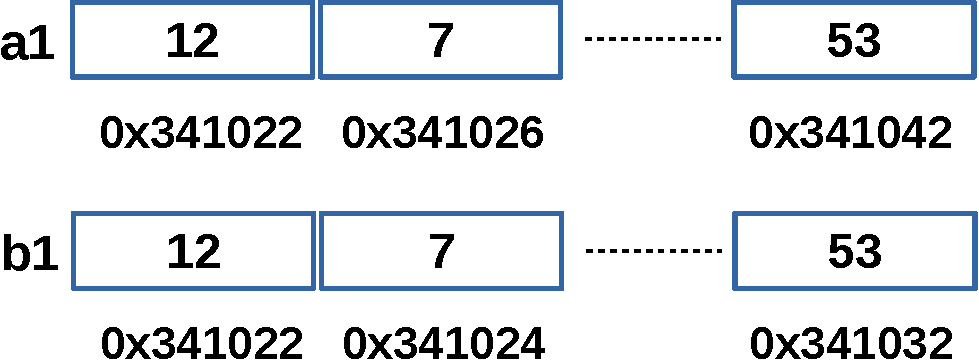
\includegraphics[width=0.57\linewidth]{figs/array1.pdf}
	\caption{Two typical arrays of \textcolor{blue}{int} type}
\end{figure}
\begin{itemize}
	\item {\textcolor{red}{Unlike} primitive type variable}
	\item {The name of an array is also the starting address of an array}
\end{itemize}
\begin{lstlisting}[xleftmargin=0.08\linewidth, linewidth=0.9\linewidth]
int main()
{
   int a[5]={4, 5, 7, 11, 13, 17};
   int *p = a;
   p = &a[0];
   return 0;
}
\end{lstlisting}
\end{frame}

\begin{frame}[fragile]{Definition and initializaiton (1)}
\begin{center}
\flushleft{
\Large{
   \textcolor{blue}{int} *p;\\
   \textcolor{blue}{int} a1[10];\\
   p = a1;\\
   p = \&a1[0];\\
}
}
\end{center}
\vspace{0.2in}
\begin{itemize}
	\item {Definition of array pointer is the same as variable pointer}
	\item {Above two ways are valid}
	\item {`\textbf{p}' keeps the address of starting address of \textbf{a1}}
	\item {Now think about what ``p = p+2' means here??}
\end{itemize}
\end{frame}

\begin{frame}[fragile]{Definition and initializaiton (2)}
\vspace{-0.15in}
\begin{lstlisting}[xleftmargin=0.1\linewidth, linewidth=0.8\linewidth]
#include <stdio.h>
int main()
{
   int a1[4] = {31, 1, 11, 4};
   int i = 0, *p = a1;
   for(i=0;i<4; i++,p++)
   {
       printf("%d ", *p);
   }
   return 0;
}
\end{lstlisting}

\begin{itemize}
	\item {`\textbf{p}' visits element in array a1 one by one}
	\item {`\textbf{*p}' takes the value according to the address in `\textbf{p}'}
\end{itemize}
\end{frame}

\begin{frame}[fragile]{Definition and initializaiton (3)}
\vspace{-0.15in}
\begin{columns}
\begin{column}{0.46\linewidth}
\begin{lstlisting}
#include <stdio.h>
int main()
{
   int a1[4]={31, 1, 11, 4};
   int i = 0, *p = a1;
   for(i=0;i<4; i++,p++)
   {
       printf("%d ", *p);
   }
   return 0;
}
\end{lstlisting}
\end{column}
\begin{column}{0.46\linewidth}
\begin{lstlisting}
#include <stdio.h>
int main()
{
   int a1[4]={31, 1, 11, 4};
   int i = 0, *p = a1;
   for(i = 0; i < 4; i++)
   {
       printf("%d ", a1[i]);
   }
   return 0;
}
\end{lstlisting}
\end{column}
\end{columns}
\begin{itemize}
	\item {`\textbf{p}' visits element in array a1 one by one}
	\item {`\textbf{*p}' takes the value according to the address in `\textbf{p}'}
\end{itemize}
\end{frame}

\begin{frame}[fragile]{Definition and initializaiton (3)}
\begin{figure}
	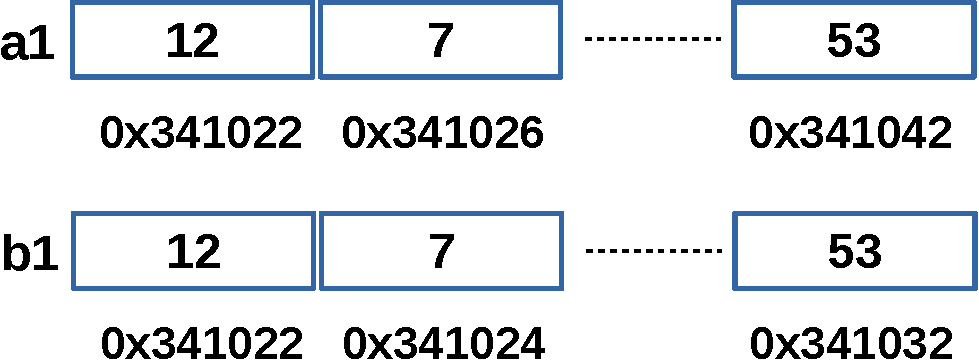
\includegraphics[width=0.50\linewidth]{figs/array1.pdf}
	\caption{Two typical arrays of \textcolor{blue}{int} type}
\end{figure}
\vspace{-0.25in}
\begin{lstlisting}[xleftmargin=0.08\linewidth, linewidth=0.9\linewidth]
int main()
{
   int a1[6] = {12, 7, 7, 11, 13, 53};
   short b1[6] = {12, 7, 7, 11, 13, 53};
   int *pa = &a1;
   short *pb = &b1;
   return 0;
}
\end{lstlisting}
\begin{itemize}
	\item {Like pointer to variable, different types of array need different types of pointer}
\end{itemize}
\end{frame}

\begin{frame}[fragile]{Operations on Pointer of Array (1)}
\begin{figure}
	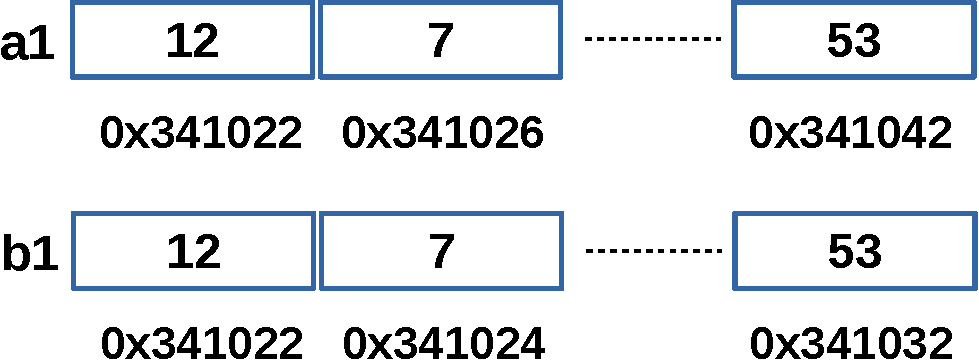
\includegraphics[width=0.48\linewidth]{figs/array1.pdf}
	\caption{Two typical arrays of \textcolor{blue}{int} type}
\end{figure}
\vspace{-0.25in}
\begin{columns}
\begin{column}{0.75\linewidth}
\begin{lstlisting}[xleftmargin=0.02\linewidth, linewidth=0.98\linewidth]
int main()
{
   int a1[6]={12, 7, 17, 11, 13, 53};
   short b1[6]={12, 7, 17, 11, 13, 53};
   int *pa = &a1;
   short *pb = &b1;
   pa++; pb++;
   printf("%d\n", *pa);
   printf("%d\n", *pb);
   return 0;
}
\end{lstlisting}
\end{column}
\begin{column}{0.20\linewidth}
[Output]\\
?\\
?
\end{column}
\end{columns}
\end{frame}

\begin{frame}[fragile]{Operations on Pointer of Array (2)}
\begin{figure}
	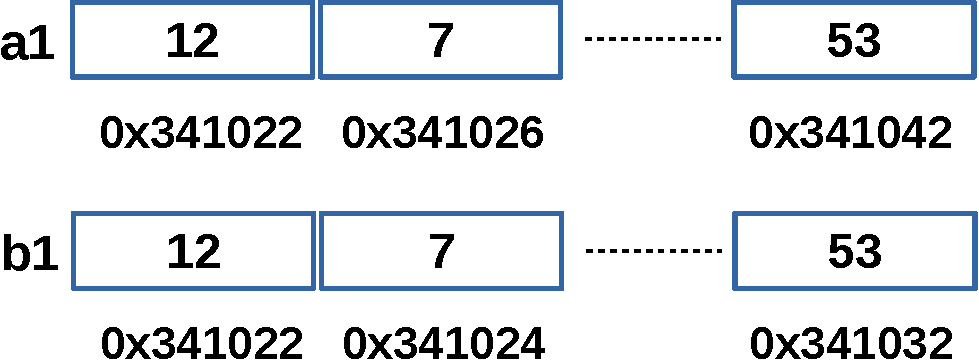
\includegraphics[width=0.48\linewidth]{figs/array1.pdf}
	\caption{Two typical arrays of \textcolor{blue}{int} type}
\end{figure}
\vspace{-0.25in}
\begin{columns}
\begin{column}{0.75\linewidth}
\begin{lstlisting}[xleftmargin=0.02\linewidth, linewidth=0.98\linewidth]
int main()
{
   int a1[5] = {12, 7, 17, 11, 13, 53};
   short b1[5] = {12, 7, 17, 11, 13, 53};
   int *pa = &a1;
   short *pb = &b1;
   pa++; pb++;
   printf("%d\n", *pa);
   printf("%d\n", *pb);
   return 0;
}
\end{lstlisting}
\end{column}
\begin{column}{0.20\linewidth}
[Output]\\
7\\
7
\end{column}
\end{columns}
\end{frame}

\begin{frame}[fragile]{Pointer to String}
\begin{itemize}
	\item {Think about following example}
	\item {We saw it many times}
	\item {Now we give a full explanation over it}
\end{itemize}
\vspace{-0.2in}
\begin{columns}
\begin{column}{0.5\linewidth}
\begin{figure}
	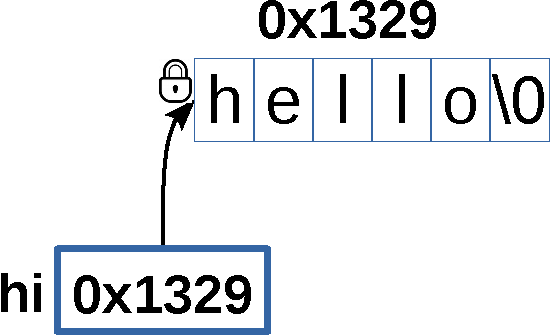
\includegraphics[width=0.55\linewidth]{figs/himem.pdf}
\end{figure}
\begin{lstlisting}[xleftmargin=0.05\linewidth, linewidth=0.95\linewidth]
#include <stdio.h>
int main()
{
   char *hi = "hello";
   hi[1] = 'a'; //<--illegal
   printf("%s\n", hi);
   return 0;
}
\end{lstlisting}
\end{column}
\begin{column}{0.5\linewidth}
\begin{figure}
	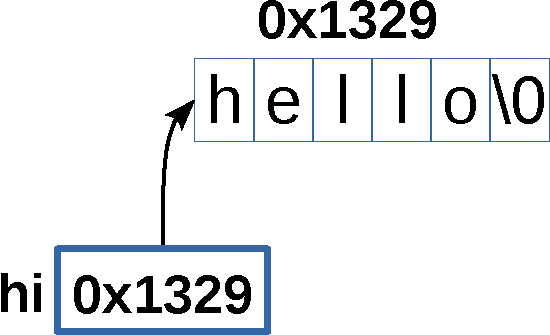
\includegraphics[width=0.6\linewidth]{figs/himem1.pdf}
\end{figure}
\begin{lstlisting}
#include <stdio.h>
int main()
{
   char hi[] = "hello";
   hi[1] = 'a'; //<--legal
   printf("%s\n", hi);
   return 0;
}
\end{lstlisting}
\end{column}
\end{columns}

\end{frame}

\begin{frame}[fragile]{Array of chars, String and Pointer of String}
\vspace{-0.15in}
\begin{itemize}
	\item {Since pointer points to the first address of an array}
	\item {``str1'' is defined as \textcolor{red}{constant} array of chars, and pointed by pointer str}
	\item {Definitions about ``str2'' and ``str3'' are \textcolor{red}{equivalent}}
	\item {Definition about ``str4'' is \textcolor{red}{different} from above three}
\end{itemize}
\begin{lstlisting}[xleftmargin=0.02\linewidth, linewidth=0.98\linewidth]
#include <stdio.h>
#include <string.h>
int main()
{
   char *str1 = "hello"; //<--str1[0] = 'a' will be illegal
   char str2[10] = "hello";
   char str3[10] = {'h', 'e' , 'l' ,'l', 'o', '\0'};
   char str4[10] = {'h', 'e' , 'l' ,'l', 'o'}; //<--it is different
   printf("%s\n", str1);
   printf("%s\n", str2);
   printf("%s\n", str3);
   printf("%s\n", str4);
   return 0;
}
\end{lstlisting}
\end{frame}

\begin{frame}[fragile]{Example of Pointer to Array (1)}
\begin{itemize}
	\item {Given \textbf{str1}="abserds" and \textbf{str2}="xxxxx"}
	\item {You are required to copy the contents of one string to another}
\end{itemize}
\end{frame}

\begin{frame}[fragile]{Example of Pointer to Array (2)}
\begin{itemize}
	\item {Given \textbf{str1}="abserds" and \textbf{str2}="xxxxx"}
	\item {You are required to copy the contents of one string to another}
	\begin{enumerate}
		\item {Define pointers (p1 and p2) for \textbf{str1} and \textbf{str2}}
		\item {Pointing to the start of each}
		\item {Assign value of p1 to p2}
		\item {Repeat \textbf{Step 3} until the end of \textbf{str1}}
		\item {Assign '$\setminus0$' to the end of \textbf{str2}}
	\end{enumerate}
\end{itemize}
\end{frame}

\begin{frame}[fragile]{Example of Pointer to Array (3)}
\begin{lstlisting}[xleftmargin=0.02\linewidth, linewidth=0.98\linewidth]
#include <stdio.h>
int main()
{
  char *str1="hello world!";
  char str2[16];
  char *p1 = str1;
  char *p2 = str2;
  while(p1 != '\0')
  {
      *p2 = *p1;
      p1++; p2++;
  }
  printf("%s\n", str1);
  printf("%s\n", str2);
  return 0;
}
\end{lstlisting}
\begin{itemize}
	\item {There is a \textcolor{red}{bug}, please tell me:)}
\end{itemize}
\end{frame}

\begin{frame}[fragile]{Example of Pointer to Array (4)}
\begin{lstlisting}[xleftmargin=0.05\linewidth, linewidth=0.95\linewidth]
#include <stdio.h>
int main()
{
  char *str1="hello world!";
  char str2[16];
  char *p1 = str1;
  char *p2 = str2;
  while(*p1 != '\0')
  {
      *p2 = *p1;
      p1++; p2++;
  }
  *p2='\0'; //<--indicate the end of the string
  printf("%s\n", str1);
  printf("%s\n", str2);
  return 0;
}
\end{lstlisting}
\vspace{-0.15in}
\begin{itemize}
	\item {Be careful all the time}
\end{itemize}
\end{frame}

\begin{frame}[fragile]{Example of Pointer to Array (5)}
\begin{lstlisting}[xleftmargin=0.05\linewidth, linewidth=0.9\linewidth]
#include <stdio.h>
void strCopy(char *p1, char *p2)
{
  while(*p1 != '\0')
  {
      *p2 = *p1;
      p1++; p2++;
  }
  *p2='\0';
}

int main()
{
  char *str1 = "hello world!";
  char str2[16];
  strCopy(?, ?);
  printf("%s\n", str1);
  printf("%s\n", str2);
  return 0;
}
\end{lstlisting}
\end{frame}

\begin{frame}[fragile]{Example of Pointer to Array (6)}
\begin{lstlisting}[xleftmargin=0.05\linewidth, linewidth=0.95\linewidth]
#include <stdio.h>
void strCopy(char *p1, char *p2)
{
  while(*p1 != '\0')
  {
      *p2 = *p1;
      p1++; p2++;
  }
  *p2='\0';
}

int main()
{
  char *str1="hello world!";
  char str2[16];
  strCopy(str1, str2);
  printf("%s\n", str1);
  printf("%s\n", str2);
  return 0;
}
\end{lstlisting}
\end{frame}

\begin{frame}[fragile]{Example of Pointer to Array (7)}
\vspace{0.1in}
\begin{figure}
	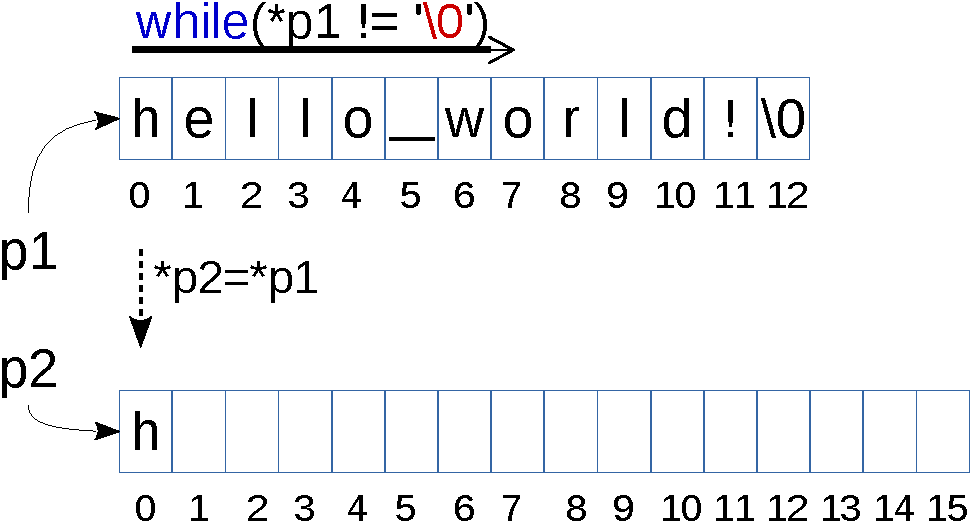
\includegraphics[width=0.8\linewidth]{figs/p2chars.pdf}
\end{figure}
\begin{itemize}
	\item {The while loop stop at '${\setminus}$0'}
	\item {'${\setminus}$0' will not be copied in the loop}
\end{itemize}
\end{frame}

\begin{frame}[fragile]{Popular functions for string operation (1)}
\begin{center}
\flushleft{
\Large{
 1. \textbf{strlen}(\textcolor{green}{str1}); length of str1, `$\setminus0$' is not counted\\
 2. \textbf{strcpy}(\textcolor{green}{str1}, \textcolor{green}{str2}); copy str2 to str1\\
 3. \textbf{strcmp}(\textcolor{green}{str1}, \textcolor{green}{str2}); compare two strings\\
 4. \textbf{strcat}(\textcolor{green}{str1}, \textcolor{green}{str2}); concantenate two strings\\
 5. \textbf{strncpy}(\textcolor{green}{str1}, \textcolor{green}{str2}, \textcolor{green}{n}); copy first \textcolor{green}{n} chars of str2 to str1
}
}
\end{center}

\end{frame}

\begin{frame}[fragile]{Popular functions for string operation (2)}

\begin{center}
\flushleft{
\Large{
 2. \textbf{strcpy}(\textcolor{green}{str1}, \textcolor{green}{str2}); copy str2 to str1\\
 4. \textbf{strcat}(\textcolor{green}{str1}, \textcolor{green}{str2}); concantenate two strings\\
}
}
\end{center}
\vspace{0.15in}
\begin{lstlisting}[xleftmargin=0.05\linewidth, linewidth=0.95\linewidth]
#include <stdio.h>
#include <string.h>
int main()
{
   char *str1="hello", *str2 = "world";
   char hi[32];
   strcpy(hi, str1);
   strcat(hi, " ");
   strcat(hi, str2);
   printf("%s\n", hi);
   return 0;
}
\end{lstlisting}
\end{frame}

\begin{frame}[fragile]{Popular functions for string operation (3)}
\vspace{-0.2in}
\begin{center}
\flushleft{
\Large{
 3. \textbf{strcmp}(\textcolor{green}{str1}, \textcolor{green}{str2}); compare two strings\\
}
}
\end{center}
\begin{lstlisting}[xleftmargin=0.05\linewidth, linewidth=0.95\linewidth]
#include <stdio.h>
#include <string.h>
int main()
{
   char *str1="hello", *str2 = "hi", *str3="hello";
   if(strcmp(str1, str2) == -1)
   {
      printf("str1 < str2!\n");
   }else if(strcmp(str1, str2) == 1) {
      printf("str1 > str2!\n");
   }
   if(strcmp(str1, str3) == 0)
   {
      printf("They are equal!\n");
   }else{
      printf("They are inequal!\n");
   }
   return 0;
}
\end{lstlisting}
\end{frame}


